\documentclass[a4paper,12pt,twoside]{report}

\usepackage[T1]{fontenc} \usepackage{lmodern} \usepackage[utf8]{inputenc}
\usepackage[english]{babel} \usepackage{csquotes}
\usepackage{float} \usepackage{graphicx,subcaption} \usepackage{subcaption}
\usepackage{amssymb,amsmath} \usepackage{siunitx}
\usepackage[style=numeric,backend=biber]{biblatex} \bibliography{refs}
\usepackage[top=4cm,bottom=4cm,left=3cm,right=3cm,headheight=15pt]{geometry}
\usepackage{fancyhdr} \pagestyle{fancy} \usepackage{lastpage}
%\usepackage{parskip} \setlength{\parindent}{0em} \setlength{\parskip}{1em}
\usepackage[colorlinks=true,allcolors=blue]{hyperref} \hypersetup{
	pdfauthor={Michaël Defferrard},
	pdftitle={Audio Classification with Structured Deep Learning},
	pdfsubject={Master project in Information Technologies}
}

%\lhead{Audio Classification with Structured Deep Learning} \chead{} \rhead{}
%\cfoot{\thepage / \pageref{LastPage}}

\usepackage[acronym]{glossaries} \makeglossaries
\newacronym{EPFL}{EPFL}{École Polytechnique Fédérale de Lausanne}
\newacronym{ICASSP}{ICASSP}{International Conference on Acoustics, Speech and Signal Processing}
\newacronym{CS}{CS}{Compressed Sensing}
\newacronym{ANNs}{ANNs}{Artificial Neural Networks}
\newacronym{CNN}{CNN}{Convolutional Neural Network}
\newacronym{RNN}{RNN}{Recursive Neural Network}
\newacronym{LSTM}{LSTM}{Long Short Term Memory}
\newacronym{MLP}{MLP}{Multi-Layer Perceptron}
\newacronym{RBM}{RBM}{Restricted Boltzmann Machine}
\newacronym{DBN}{DBN}{Deep Belief Network}
\newacronym{MIR}{MIR}{Music Information Retrieval}
\newacronym{MGR}{MGR}{Music Genre Recognition}
\newacronym{PSD}{PSD}{Predictive Sparse Decomposition}
\newacronym{CQT}{CQT}{Constant-Q Transform}
\newacronym{LCN}{LCN}{Local Contrast Normalization}
\newacronym{SVM}{SVM}{Support Vector Machine}
\newacronym{RIP}{RIP}{Restricted Isometry Property}
\newacronym{BP}{BP}{Basis Pursuit}
\newacronym{FISTA}{FISTA}{Fast Iterative Shrinkage-Thresholding Algorithm}
\newacronym{ADMM}{ADMM}{Alternating Direction Method of Multipliers}
\newacronym{PD}{PD}{Primal-Dual}
\newacronym{SGD}{SGD}{Stochastic Gradient Descent}
\newacronym{GPU}{GPU}{Graphical Processing Unit}
\newacronym{LASSO}{LASSO}{Least Absolute Shrinkage and Selection Operator}
\newacronym{AGC}{AGC}{Automatic Gain Control}
\newacronym{kNN}{kNN}{k Nearest Neighbors}

\newcommand{\eqnref}[1]{(\ref{#1})}  % Eqn~(\ref{#1})
\newcommand{\figref}[1]{Figure~\ref{#1}}
\newcommand{\tabref}[1]{Table~\ref{#1}}
\newcommand{\secref}[1]{Section~\ref{#1}}
\newcommand{\chapref}[1]{Chapter~\ref{#1}}
\newcommand{\HRule}{\rule{\linewidth}{0.5mm}}

\newcommand{\R}{\mathbb{R}}
\DeclareMathOperator*{\argminop}{arg\,min}
\DeclareMathOperator*{\minimizeop}{minimize}
\DeclareMathOperator*{\sgn}{sgn}
\DeclareMathOperator*{\tr}{tr}
\newcommand{\argmin}[1]{\argminop\limits_{#1}}
\newcommand{\minimize}[1]{\minimizeop\limits_{#1}}  % or \min
\newcommand{\normT}[1]{\| #1 \|_2^2}
\newcommand{\normO}[1]{\| #1 \|_1}
\newcommand{\normZ}[1]{\| #1 \|_0}
\newcommand{\normF}[1]{\| #1 \|_\text{F}^2}
\newcommand{\inner}[2]{\langle #1 , #2 \rangle}
\renewcommand{\L}{\mathbf{L}}
\newcommand{\D}{\mathbf{D}}
\newcommand{\E}{\mathbf{E}}
\newcommand{\X}{\mathbf{X}}
\newcommand{\Z}{\mathbf{Z}}
\renewcommand{\d}{\mathbf{d}}
\newcommand{\e}{\mathbf{e}}
\newcommand{\x}{\mathbf{x}}
\newcommand{\y}{\mathbf{y}}
\newcommand{\z}{\mathbf{z}}
\newcommand{\Eone}{E_1(\Z, \D)}
\newcommand{\Etwo}{E_2(\Z, \D, \E)}
\newcommand{\Ethree}{E_3(\Z, \D, \E)}
\newcommand{\G}{\mathcal{G}}
\newcommand{\V}{\mathcal{V}}
\newcommand{\set}[2]{\{#1_i\}_{i=1}^#2}
\newcommand{\st}{\text{ s.t. }}
\newcommand{\cst}[2]{\|#1_#2\|_2 \leq 1}
%\newcommand{\forallx}[2]{\forall #1 \in \{1,\ldots,#2\}}
\newcommand{\forallx}[2]{#1 = 1, \ldots, #2}
%\newcommand{\forallx}[2]{\|#1_#2\|_2 \leq 1 \text{ for } #2 = 1,\ldots,#3}
\newcommand{\cstd}{\cst{\d}{i}, \forallx{i}{m}}
\newcommand{\cste}{\cst{\e}{k}, \forallx{k}{n}}
\newcommand{\pd}[2]{\frac{\partial #1}{\partial #2}}

\begin{document}

\hypersetup{pageanchor=false}
\begin{titlepage}
	
	\includegraphics[height=2.5cm]{img/logo_epfl}
	\hfill
	\includegraphics[height=2.5cm]{img/logo_lts2}
	\vspace{1.5cm}
	
	\begin{center}
		
		\textsc{\LARGE MASTER THESIS}\\
		\vspace{0.5cm}
		\large Electrical and Electronic Section\\
		\large Major in Information Technologies\\
		\vspace{1.3cm}
		
		\HRule
		\vspace{1.0cm}
		\textsc{\Huge Audio Classification with}\\
		\vspace{0.7cm}
		\textsc{\Huge Structured Deep Learning}\\
		\vspace{0.6cm}
		\HRule
		\vspace{1.3cm}
		
		\begin{minipage}{0.45\textwidth}
			\begin{flushleft} \large
				\textbf{Student}\\ \vspace{0.5ex}
				Michaël \textsc{Defferrard} \\ \vspace{2.5ex}
				\textbf{Professor} \\ \vspace{0.5ex}
				Pierre \textsc{Vandergheynst}
			\end{flushleft}
		\end{minipage}
		\begin{minipage}{0.45\textwidth}
			\begin{flushright} \large
				\textbf{Supervisors} \\ \vspace{0.5ex}
				Xavier \textsc{Bresson} \\ \vspace{0.2ex}
				Johan \textsc{Paratte}
			\end{flushright}
		\end{minipage}
		
	\end{center}
	
	\vspace{1.3cm}
	{\large Conducted at the EPFL LTS2 laboratory.}
	\vspace{1.3cm}

	\begin{center}
		{\large June 19, 2015}
	\end{center}
	
\end{titlepage}
\hypersetup{pageanchor=true}

\begin{abstract}
	In this work, we present a technique to learn discriminative audio features for \gls{MIR} in an unsupervised and hierarchical way. We introduce a novel deep architecture composed by (stacks of) structured sparse auto-encoders which leverage on the recent advances of deep learning using efficient auto-encoder strategy that simultaneously learned sparse representation of inputs and dictionary adapted to those inputs. Our main goal is to find a solution to sparse coding that is structured by the proximities of the sparse features encoded by a graph of audio inputs. We borrow ideas from manifold learning to constrain our solution to be smooth on this graph, i.e. to have a small Dirichlet energy, in order to implicitly force feature proximities. Our auto-encoder model is formulated as a non-convex optimization problem, for which a {\color{red}well-posed} iterative scheme is provided. We show that the learned features combined with a simple linear classifier achieve {\color{red}110\%} accuracy in predicting genres on GTZAN.
\end{abstract}

\renewcommand{\abstractname}{Acknowledgements}
\begin{abstract}
	Xavier for day-to-day supervision. Many inputs and intuitions. Discussion of the results.
	
	Johan for intuitions at the start of the project, advices and proof reading of the thesis.
	
	Pierre
	%C’est grâce à vous que je suis satisfait de conclure ce travail éternellement inachevé par cette petite note personnelle dans une langue que je chéris beaucoup.
	
\end{abstract}

%\clearpage
%\setcounter{page}{2}
\tableofcontents

\printglossaries
\addcontentsline{toc}{chapter}{Glossary}
\addcontentsline{toc}{chapter}{Acronyms}

\chapter*{Introduction}
\addcontentsline{toc}{chapter}{Introduction}

{\color{red} Introduction to subject.}

This work was accomplished as a Master thesis, which is an integral part of the major in Information Technologies curriculum from the Electrical and Electronic Section of the \gls{EPFL}. It was conducted at the LTS2 laboratory\footnote{The laboratory homepage is accessible at \url{http://lts2www.epfl.ch/}.}.

While the project was ongoing, I continuously published my thoughts, observations, findings, experiments, results and plans as well as a summary of the weekly meetings with my supervisors on an online blog\footnote{My research blog is available at \url{https://lts2research.epfl.ch/blog/mdeff/}.} in the format of an open laboratory notebook\footnote{\url{http://en.wikipedia.org/wiki/Open_notebook_science}}. The code, as well as the results, this report and the ongoing paper is versioned with git and available online through GitHub\footnote{My GitHub account can be found at \url{https://github.com/mdeff}.}. A continuation of this work shall be submitted to the 41st IEEE \gls{ICASSP}.

This thesis is divided in two parts: 

\section*{Motivation}
\addcontentsline{toc}{section}{Motivation}

\section*{Background}
\addcontentsline{toc}{section}{Background}

\section*{Related work}
\addcontentsline{toc}{section}{Related work}
% LeCun's paper

Similarly to us, the authors of \cite{lecun2011PSDaudio} used a layer of sparse auto-encoder to learn sparse representations of audio spectrograms. They introduced a technique called \gls{PSD} to quickly infer an approximation of the sparse codes \cite{lecun2010PSD}.

In this work, we generalize their loss function as an energy function and introduce a structuring term. We also introduce a well-posed iterative scheme to solve the resulting non-convex optimization problem.

\part{Theoretical foundations}
% Explain the methods we'll later use.

\chapter{Music theory}
% Explain how music is constructed.

\section{Notes and frequencies}

\section{Harmonics, chords and harmonies}

\section{Constant-Q transform}
% Spectrogram with geometrically spaced frequencies.

\section{Genres}
% How we can qualitatively distinguish genres.

\chapter{Machine learning}
% What's the purpose of learning.
% Why learned features instead of hand-crafted features ?

\section{Supervised vs unsupervised}
% Explain the difference. Why do we want unsupervised ?

\section{Feature / representation learning}
% NN is well suited for representation learning
% We want unsupervised feature learning vs supervised vs hand-crafted

\section{Support Vector Machine}
% Used for classification

\section{Sparse coding} \label{sec:sparse_coding}
% What it is, why it works, why it's good.
% paper who demonstrates that L1 penalty leads to same solution as L0 while being convex, not combinatorial

% Sparse coding.
Sparsity has become a concept of great interest recently, not only in
machine learning but also in statistics and signal processing, in particular with the work on compressed sensing \cite{candes2005CS, donoho2006CS}. The main idea behind sparse coding {\color{red} [ref]} is to express a signal $\x \in \R^n$ as a sparse linear combination of basis functions $\set{\d}{m}$, or atoms, from an overcomplete ($m>n$) dictionary $\D \in \R^{n \times m}$. The sparse code $\z^* \in \R^m$ is given by
\begin{equation}\label{eqn:sparsecoding}
	\z^* = \argmin{\z} \frac{\lambda_d}{2} \normT{\x - \D \z} + \lambda_z \normZ{\z}
\end{equation}
where $\normZ{\z}$ denotes the number of non-zero elements in $\z$ and $\normT{\cdot}$ the squared $\ell_2$, or Euclidean, norm. $\lambda_d$ and $\lambda_z$ are the (redundant) hyper-parameters setting the trade-off between the data term (an accurate reconstruction) and the prior (a sparse solution). Overcomplete sparse representations tend to be good features for classification systems as they provide a succinct representation of the signal, are robust to noise and are more likely to be linearly separable due to their high dimensionality.

% Faster sparse coding approximations.
Finding the sparse code $\z^*$ however requires a combinatorial search which is an NP-hard problem, intractable in high dimensional spaces. Various approximations have thus been proposed. Matching Pursuit \cite{mallat1993MatchingPursuit} offers a greedy approximation to the solution while \gls{BP} \cite{chen1998BasisPursuit} is the popular convex approximation
\begin{equation}\label{eqn:basispursuit}
	\z^* = \argmin{\z} \frac{\lambda_d}{2} \normT{\x - \D \z} + \lambda_z \normO{\z}
\end{equation}
where $\normO{\z} = \sum_{i=1}^{m} |z_i|$ is the $\ell_1$ norm of $\z$ (also called the Taxicab or Manhattan norm). As is now well understood \cite{candes2005CS, donoho2006CS}, the $\ell_1$ norm is a very good proxy for the $\ell_0$ norm and naturally induces sparse results. It can even be shown to recover exactly the true sparse code, i.e. the solution of \eqnref{eqn:sparsecoding} (if there is one), under mild conditions \cite{donoho2003OptSparse}. {\color{red}link with \gls{RIP}}. A number of algorithms have been proposed to efficiently solve this problem \cite{chen1998BasisPursuit, beck2009FISTA, ng2006EfficientSparse, li2009Coordinate} {\color{red} [others]}. They however still rely on computationally expensive iterative procedures which limit the system's scalability and real-time applications. While a direct method will always be preferred for feature extraction, iterative methods will still be necessary during training. Distributed computing with \gls{GPU} or via cloud computing will hopefully accelerate the process.

\subsection{Dictionary learning}

% Why ?
In classical sparse coding, the dictionary is composed of known functions such as sinusoids, gammatones, wavelets or Gabors; i.e. hand-crafted features. One may also want to learn a dictionary that is adaptive to the type of data at hand. This approach allows an even more compact representation and may lead to the discovery of previously unknown discriminative features.

% How ?
To use the dictionary $\D$ as an unknown variable, we shall integrate all the training data into the objective function as the dictionary depends on all of them. The energy function, composed by an $\ell_2$ fidelity term and an $\ell_1$ penalty, becomes
\begin{equation}\label{eqn:en_dict}
	\Eone = \frac{\lambda_d}{2} \normF{\X - \D \Z} + \lambda_z \normO{\Z}
\end{equation}
where $\normF{\cdot}$ denotes the squared Frobenius norm, $\X = \set{\x}{N} \in \R^{n \times N}$ is the set of training vectors and $\Z = \set{\z}{N} \in \R^{m \times N}$ their associated sparse codes. $N$ is naturally the number of training vectors, which should be much greater than the size $m$ of the dictionary to avoid the trivial solution where examples are copied in the dictionary. The problem to solve is then
\begin{equation}\label{eqn:pr_dict}
	\minimize{\Z,\D} \Eone \st \cstd
\end{equation}
where the constraint (usually implemented by rescaling the columns $\d_i$ of $\D$ at each iteration) prevents the trivial solution where the code coefficients go to zero while the bases are scaled up. While this problem is not convex, an approximate solution can be found by iteratively minimizing for $\Z$ and $\D$ \cite{olshausen1996SparseV1}.
% Simple gradient descent or more sophisticated methods \cite{chen1998BasisPursuit, beck2009FISTA, li2009Coordinate} for $\z$, stochastic gradient descent for $\D$.

% Motivation: learned dictionaries resemble brain processing stages.
There is evidence that sparse coding may be a strategy employed by the brain in the early stages of visual and auditory processing \cite{olshausen1996SparseV1, olshausen1997SparseV1, smith2006SparseAudio}. Basis functions learned on natural images have been shown to resemble the receptive fields of neurons in the visual cortex \cite{olshausen1996SparseV1, olshausen1997SparseV1}. Basis functions learned on natural sounds were found to be highly similar to gammatone functions \cite{smith2006SparseAudio} which have been used to model the action of the basilar membrane in the inner ear. Moreover, learning on natural time-varying stimuli such as speech or video has been shown to produce localized bases \cite{lewicki2000SparseSpeech, olshausen2000SparseVideo}.

\paragraph{Completeness}
Note that a dictionary can be either complete ($m=n$), undercomplete ($m<n$) or overcomplete ($m>n$).
Examples of complete dictionaries are bases, like the Fourier transform, which allow lossless transformations.
Undercomplete dictionaries are good for dimensionality reductions as they exploit the statistical regularities present in the training set. As there is then no solution to $\x = \D\z$, an error measure like $\normT{\x - \D\z}$ should instead be minimized.
Overcomplete dictionaries are good for classification as they allow for an easier (linear) separability enabled by the higher dimensional space. As there is then an infinite number of solutions to $\x = \D\z$, we shall introduce a regularization over $\z$. Optimization techniques are then used to find the optimal solution which minimizes the sum of the error measure and the regularization term, controlled by an hyper-parameter.
% overcompleteness must be evaluated by considering the number of code units and the effective dimensionality of the input as given by PCA

\paragraph{Regularization}
The Tikhonov regularization, or ridge regression, is a commonly used prior of the form $\lambda \normT{\mathbf{\Gamma} \z}$ where $\mathbf{\Gamma}$ is the Tikhonov matrix. This matrix is often chosen to be a multiple of the identity matrix, i.e. $\mathbf{\Gamma} = \alpha \mathbf{I}$, giving preference to solutions with smaller norms. In a Bayesian context, this is equivalent to placing a zero-mean normally distributed prior on $\z$. In other cases, lowpass operators (e.g., a difference operator or a weighted Fourier operator) may be used to enforce smoothness if the underlying vector is believed to be mostly continuous. We will introduce a regularization of this kind to our model in \secref{sec:graph_regularization}.
Another commonly used regularization is the \gls{LASSO}, which adds the term $\lambda \normO{\z}$ to the minimization problem \cite{tibshirani1996Lasso}. In a Bayesian context, this is equivalent to placing a zero-mean Laplace prior distribution on $\z$ \cite{park2008BayesianLasso}. As we have seen in \ref{sec:sparse_coding}, we use this prior in our model to enforce sparsity. The advantage of the \gls{LASSO} is that it promotes the simplest solutions, i.e. the solutions with many zeros. Driving parameters to zero effectively deselects the features from the regression. \gls{LASSO} thus automatically selects the most relevant features, whereas ridge regression never fully discards any. For this reason, the \gls{LASSO} and its variants are fundamental to the field of \gls{CS}.
An extension of this approach is the elastic net regularization which linearly combines the $\ell_1$ and $\ell_2$ penalties of the \gls{LASSO} and ridge methods. This regularization overcomes some limitations of the $\ell_1$ penalty, e.g. the saturation which happens for high-dimensional data with few examples, or the fact that the \gls{LASSO} tends to select only one variable and ignore the others if there is a group of highly correlated variables \cite{zou2005ElasticNet}.

\subsection{Encoder} \label{sec:encoder}
% Problem: these methods are slow at inferring sparse codes as they need iterations
% --> train an encoder
{\color{red} Put after sparse auto-encoders ? Because it is our definition of a sparse auto-encoder.}

% Why ?
In order to avoid the iterative procedure typically required to infer the sparse code, we aim at an encoder which can quickly map inputs to approximations of their sparse code. Several works \cite{lecun2010PSD, lecun2010LISTA, lecun2013DrSAE} {\color{red} [others not from LeCun]} has been done in this direction. The addition of an encoder to the sparse coding scheme leads to a variant of auto-encoders called sparse auto-encoders which we will introduce in \ref{sec:auto_encoders}.

% 2nd motivation.
Moreover, adding structure to the problem should enhance the behavior of the loss function and help sparse recovery \cite{kowalski2009sparse, baraniuk2010modelCS, huang2011LearningStructuredSparsity, jenatton2011structured} {\color{red}Then \cite{donoho2003OptSparse} should not be strong enough.}

% How ?
Introducing a trainable encoder $\E \in \R^{m \times n}$ into our model gives the energy function
\begin{equation}\label{eqn:en_encoder}
	\Etwo = \Eone + \frac{\lambda_e}{2} \normF{\Z - \E \X} {\color{red} + \lambda_s \normO{\E \X}}
\end{equation}
where $\lambda_e$ and $\lambda_s$ are two additional hyper-parameters which control the sparsity versus fidelity tradeoff. The problem is then defined by
\begin{equation}\label{eqn:pr_encoder}
	\minimize{\Z,\D,\E} \Etwo \st \cst{\d}{i} , \cst{\e}{k} ,
	\forallx{i}{m} , \forallx{k}{n}
\end{equation}
where $\e_k$ are the columns of $\E$. Again, the $\ell_1$ penalty $\normO{\E \X}$ regularizes the least square problem, i.e. the \gls{LASSO} method.

While it is often a good idea to control the energy, the constraint on the columns of $\E$ is not needed in practice. While the columns of $\D$ are constrained to a norm smaller than one, they are in practice normalized because of the $\normO{\Z}$ objective. The energy of a vector transformed by $\D$ does thus not change, which means that the inferred sparse code $\z_i$ as the same energy as its corresponding vector $\x_i$. The encoder does then not need to add energy and will have a column norm smaller than one, even without the constraint. It has been verified in practice, see {\color{red} Fig}.

\section{Neural networks}
% Why ? Distributed representation and computation (e.g. training on GPU, clusters) --> much what symbolic AI is not (mainly search algorithms, SAT solvers)
% Started in the late 1950s with the perceptron.

\gls{ANNs} are a family of statistical learning models inspired by biological neural networks and are used to estimate or approximate functions that can depend on a large number of inputs and are generally unknown. It is presented as a network of interconnected neurons whose connections have numeric weights that can be tuned based on experience. It makes the neural nets adaptive to inputs and capable of learning.

% What is it ? In general.
Such a network is composed by an input layer, a number of hidden layers and an output layer. The activation of the neurons in the input layer corresponds to the input vector, e.g. an image for computer vision, a song for \gls{MIR}, a word vector for machine translation and sentiment analysis. A weight matrix, followed by a non-linear activation function, then transforms the vector in another representation. The output vector of the first layer is the input vector of the second, and so on until the output layer is reached. The activation of the neurons in the output layer may represent classes, probability distributions, or the estimated value of an unknown function to be learned.

{\color{red} Picture ?}

% Types: feed-forward or recurrent
In a feed-forward network, the connections go from one layer to the next, i.e. information only goes in one direction, forward, from the input nodes, through the hidden nodes (if any) and to the output nodes. Such networks are known to be able to approximate any function. The perceptron, the \gls{MLP} and the \gls{CNN} are examples of this class of networks.
By introducing backward connections, i.e. the connections between units form a directed cycle, we obtain a so called \gls{RNN}. This creates an internal state of the network which allows it to exhibit dynamic temporal behavior. Unlike feed-forward neural networks, an \gls{RNN} can use its internal memory to process arbitrary sequences of inputs. It is known to be able to approximate any program. Such networks have proven very successful for machine translation.

% How to train, supervised.
In a supervised learning setting, the network is trained by back-propagating the error, gradient based learning method, from the output layer to the input through all the hidden layers.
The vanishing gradient problem, where errors shrink exponentially with the number of layers as they propagate from layer to layer, is a major issue of the algorithm \cite{hochreiter2001vanishingGradient}. Various methods, like unsupervised pre-training or \gls{LSTM} \cite{hochreiter1997LSTM}, were developed to work around this problem.

% How to train, unsupervised.
However, in an unsupervised learning setting, there is no desired output, which implies that there is no error to back-propagate. The training algorithm should thus optimize for another objective, which represent desired properties about the output. We will introduce next such an algorithm, called an auto-encoder.

\subsection{Auto-encoders} \label{sec:auto_encoders}
% For unsupervised learning, i.e. feature extraction.
% Auto-encoders as a manifold learning tool (Bengio review).

An auto-encoder, auto-associator or Diabolo network is an artificial neural network composed of $n$ input and output units and $m$ hidden units. It is used for learning efficient codings \cite{bourlard1988autoencoder, hinton1994autoencoder}. The aim of an auto-encoder is to learn a distributed representation (encoding) for a set of data. An auto-encoder is trained to encode the input $\x \in \R^n$ into some representation $\z \in \R^m$ so that the input can be reconstructed from that representation. It is thus a generative model. Hence the target output of the auto-encoder is the auto-encoder input itself. Auto-encoders may further be stacked to form a \gls{DBN}, while each layer can be trained separately \cite{bengio2007DBN, lecun2006stackedSparseAutoencoders}.
% Stacked Auto-Encoders, not DBN

{\color{red} Picture ?}

% if linear activations are used, or only a single sigmoid hidden layer, then the optimal solution to an auto-encoder is strongly related to principal component analysis (PCA).[5]
If there is one linear hidden layer and the mean squared error criterion is used to train the network, then the $k$ hidden units learn to project the input in the span of the first $k$ principal components of the data \cite{bourlard1988autoencoder}. If the hidden layer is non-linear, the auto-encoder behaves differently from PCA, with the ability to capture multi-modal aspects of the input distribution \cite{japkowicz2000autoencoderPCA}.

The hope is that the code $\z$ is a distributed representation that captures the main factors of variation in the data: because $\z$ is viewed as a lossy representation of $\x$, it cannot be a good representation (with small loss) for all $\x$. So learning drives it to be one that is a good representation in particular for training examples, and hopefully for others as well (and that is the sense in which an auto-encoder generalizes), but not for arbitrary inputs.

It can typically be used for dimensionality reduction by learning a compressed ($m<n$) representation of the data. Another application is feature extraction before classification, for which we want an higher dimensionality ($m>n$) for easier separability. One serious issue with this approach is that if there is no other constraint, then an auto-encoder with $n$-dimensional input and an encoding of dimension $m \geq n$ could potentially just learn the identity function. There are different ways that an auto-encoder with more hidden units than inputs could be prevented from learning the identity, and still capture something useful about the input in its hidden representation $\z$.

\paragraph{Denoising auto-encoders}
One strategy is to add noise in the encoding. The denoising auto-encoder thus minimizes the error in reconstructing the input from a stochastically corrupted transformation of the input \cite{bengio2008denoisingAutoencoders}. Intuitively, a denoising auto-encoder does two things: try to encode the input (preserve the information about the input), and try to undo the effect of a corruption process stochastically applied to the input of the auto-encoder. This is essentially what a \gls{RBM} does \cite{hinton2002RBM}.

\paragraph{Sparse auto-encoders}
Another strategy, based on the concept of sparse coding, is to add a sparsity constraint on the code. While an ordinary auto-encoder or an \gls{RBM} has an encoder part which computes $P(\z|\x)$ and a decoder part which computes $P(\x|\z)$, sparse coding systems only parametrize the decoder: the encoder is defined implicitly as the solution of an optimization. A middle ground between ordinary auto-encoders and sparse coding was proposed in \cite{lecun2006stackedSparseAutoencoders, ranzato2007stackedSparseAutoencoders} and applied to pattern recognition and machine vision tasks. They propose to let the codes $\z$ be free (as in sparse coding algorithms), but include a parametric encoder (as in an ordinary auto-encoder or \gls{RBM}) and a penalty for the difference between the free non-parametric codes $\z$ and the outputs of the parametric encoder. In this way, the optimized codes $\z$ try to satisfy two objectives: reconstruct well the input (like in sparse coding), while not being too far from the output of the encoder (which is stable by construction, because of the simple parametrization of the encoder). See \secref{sec:encoder} for the definition of our encoder.

\subsection{Deep learning}
% Rebranded as deep learning, achieve now astonishing results in a variety of fields (computer vision, NLP, machine translation, knowledge representation, automatic control)
% Deep learning: hierarchical feature learning --> we are not really using that (yet)
% Deep architectures can approximate any function (RNN any program, i.e. Turing complete)
% First fall of NN (success of kernel methods / SVM) (first AI winter ?) because perceptron was proved to not be sufficient, multi-layer was too hard (computation and training)
% Computationally expensive to train
% Needed to invent backpropagation to train multiple layers
% Hard to train: problem of vanishing gradient
% Objective function is highly non-convex.
% popularized by CNN.

% DBN: stacks of RBM
% Stacked auto-encoders

\chapter{Convex optimization}

\section{Convex problem}
% What is a convex problem (objective and constraints).
% Methods to solve: analytically or numerical schemes.

\section{Numerical solvers}
% Numerical: gradient descent --> slow --> second order methods like Newton
% Stochastic gradient descent

\section{Proximal splitting methods}
% But our objective function is not differentiable
% Ridge regression is, but not the LASSO regularization.
% --> rely on a sub-gradient method, the proximity / proximal operator --> proximal splitting

\subsection{Forward-backward}
% Different basic methods to solve these problems: forward-backward, douglas-rachford
% Explain the intuition

\subsection{Douglas-Rachford}

\subsection{FISTA}
% Advanced (faster) algorithms who exlpoit variable time steps and multiple points: FISTA

\section{Dual problem}
% Introducing the dual problem (paper playing with duality)

\subsection{Primal-dual}

\chapter{Spectral graph theory}
% Paper: Pierre's review

%\section{Graph definition}
% What is a graph --> discrete approximation of a low-dimensional manifold embedded in a high dimensional space.

% General formulation.
Graphs are generic data representation forms which are useful for describing the geometric structures of data domains in numerous applications, including social, energy, transportation, sensor, and neuronal networks. The connectivity and weight associated with each edge in the graph is either dictated by the physics of the problem at hand or inferred from the data; in which case it often represents the similarity between the two vertices it connects. For instance, the edge weight may be inversely proportional to the physical distance between nodes in the network, or proportional to a similarity measure between those nodes. A \textit{graph signal} is a signal which resides on the graph, i.e. a signal with one sample at each vertex of the graph. An example of a graph signal is shown in \figref{example_graph}.

\begin{figure}[ht]
	\centering
	\includegraphics[height=6cm]{img/example_graph}
	\caption[]{A random positive graph signal on the vertices of the Petersen graph. The height of each blue bar represents the signal value at the vertex where the bar originates.\footnotemark}
	\label{example_graph}
\end{figure}
\footnotetext{Image from \cite{pierre2013graph}.}

Weighted graphs are commonly used to represent similarities between data points in statistical learning problems for applications such as machine vision
[2] and automatic text classification [3].

We first review some basic definitions and notations from spectral graph theory and then show how we can use a graph to approximate a manifold.

\subsection{Weighted Graphs and Graph Signals}


A graph $\G$

\subsection{Type}
% Type of graph (KNN vs epsilon)

\subsection{Distance metric}
% euclidean (small dim) and cosine (angular, high dim)

\subsection{Kernel}
% Gaussian or polynomial

\section{Spectrum}
% What does the spectrum / Fourier transform mean: examples on a 3D point cloud.
% Faster way to compute FT: Chebyshev approximation (filter bank)
% We do not use that.

There is more to spectral graph theory than what we use in this project. A number of transform methods, like the Fourier or wavelet transforms, have been defined on arbitrary graphs. Common data processing tasks in these applications include filtering, denoising, inpainting, and compressing graph signals.


\section{Laplacian}
% The graph (normalized) Laplacian is an approximation of the Laplace-Beltrami operator. --> Dirichlet energy
% normalized vs un-normalized, cite normalized approximates the Laplace-Beltrami operator
% A way to test if the Laplacian is well constructed is... (see blog)
% Another regularization on Z. Like Thikonov with the graph Laplacian as the Tikhonov matrix (difference operator). It enforces smoothness on the graph / manifold.

\section{Manifold approximation}

% General introduction.
In mathematics, a manifold is a topological space that resembles Euclidean space near each point, i.e. each point of an $n$-dimensional manifold has a neighborhood that is homeomorphic to the Euclidean space of dimension $n$. Lines and circles, but not figure eights, are one-dimensional manifolds. Two-dimensional manifolds are also called surfaces. Examples include the plane, the sphere, and the torus, which can all be embedded in three-dimensional real space. \figref{fig:manifolds} shows examples of 1D and 2D manifolds.

\begin{figure}[ht]
	\centering
	\begin{subfigure}[b]{0.49\textwidth}
		\centering
		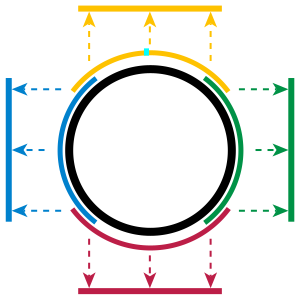
\includegraphics[height=6cm]{img/circle_manifold_charts}
		\caption{}
	\end{subfigure}
	\begin{subfigure}[b]{0.49\textwidth}
		\centering
		\includegraphics[height=6cm]{img/klein_bottle}
		\caption{}
	\end{subfigure}
	\caption[]{Examples of manifolds.\footnotemark (a) The circle, a 1D manifold, can be mapped by 4 charts. (b) The klein bottle is a 2D manifold that cannot be embedded in a 3D space without self-intersection.}
	\label{fig:manifolds}
\end{figure}
\footnotetext{Images from Wikipedia.}

% Example close to our case.
Let's imagine a single handwritten digit recognition system. The input is an image of $n \times n$ pixels which is represented by a vector $\x \in \R^{n \times n}$. However, not all vectors $\x \in \R^{n \times n}$ represent meaningful data. The vast majority indeed represents garbage. We may make the hypothesis that the set of plausible digits lies on a $d$-dimensional manifold where $d \leq n \times n$.

% Approximate a manifold.
The problem is that we often ignore the shape of the embedded manifold. We only have at our disposal some samples which are drawn from it, e.g. a few examples of handwritten digits. Another example with object scanning: we obtain a discrete point cloud sampled from the surface. We do know some points on the surface, but we don't know the exact surface.

We use graphs as discrete approximations of low-dimensional manifolds embedded in high-dimensional spaces. The set of data are samples drawn from this unknown manifold.

\section{Regularization} \label{sec:graph_regularization}

\part{Contributions} \label{part:contributions}
% Proposed method / method
% Based on the introduced methods, explain what we did.

\chapter{Model} \label{chap:model}
% Visual diagram: pre-processing, feature extraction, post-processing, classification
% energy-based model

\section{Hypothesis}

% (Known) hypothesis: patches of spectrogram are composed by a linear combination of atoms. These atoms form a dictionary. As we shall see, these atoms represent harmonies, harmonics, drums etc.

% (New) hypothesis: audio spectrograms lie on a low-dimensional manifold embedded in a high dimensional space.
% Structured: adding similarity information between inputs
% Manifold: not all possible signals are reasonable / feasible

\section{Model}

% Finish with the complete objective function.
% Why energy function ? Many laws of nature are nothing but optimality conditions, often expressed in terms of a minimum energy principle.
% Easy to add and remove terms.
% the sparsity constraint prevents the auto-encoder to learn the identity

{\color{red} Image with input x and hidden z. Output is y=sh(Ex). Weight matrices are D and E with sh() activation function. Approximately.}

% Sparse coding: terms ..
% Auto-encoders: terms ..
% Manifold learning: terms ..
% Regularized least square (elastic net): terms ..

In our genre recognition setting, a patch spectrogram\footnote{We will define it precisely in \chapref{chap:model}, think of it as the spectrogram of some short time frame.} $\x \in \R^n$ is embedded in an $n$-dimensional space. Not all $n$-dimensional signals, however, are plausible spectrograms. We may think of the set of plausible spectrograms to lie on a lower $k$-dimensional manifold which is embedded in the $n$-dimensional space.

Our overall model may be thought as an hybrid between a sparse and a denoising auto-encoder.

\section{Graph construction}
% Similarity measure
% KNN graph

\section{Problem formulation}
% Construction: sparse coding, dictionary learning, encoder learning, manifold learning
% Non-convex problem composed of convex sub-problems.
% Derive prox and gradients.
% Why we can use FISTA an PD ?
% Derive FISTA and primal-dual formulations.

\section{Training}
% Batch (FISTA, primal-dual) and online (stochastic gradient descent) training
% Transductive learning

\section{Feature extraction}
% Most accurate extraction with original model.
% Much faster approximations by ignoring some terms of the objective.

\section{Audio pre-processing}
% Frames, CQT, LCN, feature / sample normalization

\section{Classification}
% Feature aggregation (feature vectors), linear SVM, majority voting (winner take all)
% Voting further gives a cheap confidence level about our choice.
% Multi-class: one-vs-one / one-vs-the-rest

\chapter{Implementation}

\section{Framework}
% Stack: numpy, scipy, matplotlib, scikit-learn, librosa
% Tools: IPython notebook, CDK cluster, matplotlib, h5py, librosa
% Explain why and how data is stored (layout) via HDF5.

\subsection{PyUNLocBoX}
% PyUNLocBoX: explains how it works

\section{Design}

\section{Performance}

\subsection{Algorithm}
% FISTA vs PD implementation

\subsection{Approximate KNN search}
% How FLANN works, what are the alternatives.
% Techniques: KDtree, ball, local hashes (LHS)

\subsection{Optimization for space}
% Optimization for space: avoid copy, modify in place, float32, store Z as scipy.sparse

\subsection{Optimization for speed}
% Optimization for speed: ATLAS/OpenBLAS, float32 (memory bandwidth), projection in the ball (not on the sphere)
% ATLAS mono-threaded (at least on Ubuntu), OpenBLAS multi-threaded.
% Linear algebra: optimized version of BLAS: ATLAS and OpenBLAS. (LINPACK)

\chapter{Results}
% Results and comparisons
% Include discussion in results ?

\section{Spectrograms}
% Show example spectrograms of jazz / blues. Show how they are different (music theory) and can such be distinguished.

\section{Learned features}
% Show some atoms: harmonics, chords, harmonies, drums.
% Probably not on full CQT, should be on octaves.

\section{Descriptive feature vectors}
% Show aggregated feature vectors for some genres.
% How is it qualitatively more discriminative than the spectrogram ?

\section{Hyper-parameters tuning}
% Test matrix for hyper-parameters on smaller problem (i.e. less frames).
% For ld, le, lg, m
% Numerical parameters: Nouter (enough when no more inner), rtol
% Graph parameters: K, Csigma, kernel?, metric
% Classification: C, Nvectors
% Pre-processing: na=1024, ns=96

\section{Classification accuracy}
% Measured via 10-fold cross-validation
% How classification is improved by feature learning, introducing the encoder / graph.
% Comparison with other techniques.

\chapter{Discussion}
% Discussion of our results. Strengths and weaknesses of our method.

\chapter*{Conclusion}
\addcontentsline{toc}{chapter}{Conclusion}

\section*{Future work}
\addcontentsline{toc}{section}{Future work}

\paragraph{Encoder}

\paragraph{LCN}
% Not if we cannot justify.

\paragraph{Individual octaves}

\paragraph{TV norm}
% TV norm on the graph instead of Dirichlet energy

\paragraph{Distributed implementation}
% Train chunks of D / Z via independant threads.
% Directly in the PyUNLocBoX ?
% Usefull only if we are not memory bandwidth limited.
% Why ATLAS does not do it by default ? OpenBLAS does it.
% Move to GPU.

\paragraph{Multiple layers}
% Multiple layers of auto-encoders

\paragraph{End-to-end learning}
% Learn features right from raw audio. If spectrograms are good features, we should retrieve them.

\paragraph{Domain knowledge}
% Incorporate some domain knowledge about the dictionary via priors. Then it's not supervised anymore.
% Priors on the dictionary who are not necessarily domain specific, i.e. are general enough to apply to other kind of data.

\printbibliography
\addcontentsline{toc}{chapter}{References}

\chapter*{Annexes}
\addcontentsline{toc}{chapter}{Annexes}

\section*{Conference paper}
\addcontentsline{toc}{section}{Conference paper}
% Draft of ISMIR / ICASSP paper

\section*{Code}
\addcontentsline{toc}{section}{Code}
% IPython notebooks exported as LaTex.
% Available on GitHub.

\end{document}